\documentclass[a4paper,UKenglish,cleveref,autoref]{lipics-v2021}

\usepackage{mathtools}
\usepackage[abbreviations]{foreign}
\usepackage[super]{nth}
\usepackage{xspace}
\usepackage{tikz}
\usepackage{minted}
\usepackage[disable]{todonotes}

\hideLIPIcs%

\bibliographystyle{plainurl}% the mandatory bibstyle

\title{Tactics modulo associativity and cancellation for category theory}

%\titlerunning{}

\author{Kazuhiko Sakaguchi}{ CNRS, ENS de Lyon, UCBL, LIP, UMR 5668, France}{kazuhiko.sakaguchi@ens-lyon.fr}{https://orcid.org/0000-0003-1855-5189}{}%TODO mandatory, please use full name; only 1 author per \author macro; first two parameters are mandatory, other parameters can be empty. Please provide at least the name of the affiliation and the country. The full address is optional. Use additional curly braces to indicate the correct name splitting when the last name consists of multiple name parts.

\authorrunning{K. Sakaguchi}

\Copyright{Kazuhiko Sakaguchi}

\ccsdesc[500]{Computing methodologies~Theorem proving algorithms}
\ccsdesc[500]{Theory of computation~Automated reasoning}
\ccsdesc[500]{Theory of computation~Type theory}
\ccsdesc[500]{Theory of computation~Constraint and logic programming}

\keywords{Rocq, Elpi, proof by reflection, category theory}

%TODO
%\relatedversion, \relatedversiondetails
%\supplement, \supplementdetails
%\funding{}
% \acknowledgements{}

\ifx\authoranonymous\relax
\else
\nolinenumbers %uncomment to disable line numbering
\fi

%Editor-only macros:: begin (do not touch as author)%%%%%%%%%%%%%%%%%%%%%%%%%%%%%%%%%%
\EventEditors{John Q. Open and Joan R. Access}
\EventNoEds{2}
\EventLongTitle{42nd Conference on Very Important Topics (CVIT 2016)}
\EventShortTitle{CVIT 2016}
\EventAcronym{CVIT}
\EventYear{2016}
\EventDate{December 24--27, 2016}
\EventLocation{Little Whinging, United Kingdom}
\EventLogo{}
\SeriesVolume{42}
\ArticleNo{23}
%%%%%%%%%%%%%%%%%%%%%%%%%%%%%%%%%%%%%%%%%%%%%%%%%%%%%%

%%%% Minted

\usemintedstyle{default}
\newminted[rocqcode]{elpi.py:RocqLexer}{fontsize=\small,linenos=true,escapeinside=\#\#,texcomments}
\newmintinline[rocq]{elpi.py:RocqLexer}{escapeinside=\#\#}
\newminted[elpicode]{elpi.py:ElpiLexer}{fontsize=\small,linenos=true,escapeinside=\#\#,texcomments}
\newmintinline[elpi]{elpi.py:ElpiLexer}{escapeinside=\#\#}

%% Math notations

\newcommand\conveq{\equiv}
\newcommand\unify{\ensuremath{\mathrel{\hat{\conveq}}}}
\newcommand\evar[1]{\ensuremath{?_{\texttt{#1}}}}

%%%% Terms

\newcommand{\Rocq}{{\sffamily\scshape Rocq}\xspace}
\newcommand{\Elpi}{{\sffamily\scshape Elpi}\xspace}
\newcommand{\RocqElpi}{{\sffamily\scshape Rocq-Elpi}\xspace}
\newcommand{\HB}{{\sffamily\scshape Hierarchy Builder}\xspace}
\newcommand{\OCaml}{{\sffamily\scshape OCaml}\xspace}

\begin{document}

\maketitle

\begin{abstract}
  We propose \Rocq tactics for equational reasoning in category theory, that enable reasoning modulo
  the common equational laws:
  associativity, \ie, $(f ; g) ; h = f ; (g ; h)$,
  identity, \ie, $\mathrm{id}; f = f = f; \mathrm{id}$, and
  cancellation, \ie, $f ; f^{-1} = \mathrm{id}$.
  Our tactics consist of two building blocks: reflexive normalisation procedures modulo equational
  laws, and matching procedures written in \RocqElpi.
  Unlike the modulo associativity and commutativity tactics of Braibant and
  Pous~\cite{DBLP:conf/cpp/BraibantP11}, our tactics support morphisms whose types are constrained
  by their source and target objects.
  The paper is written as a tutorial, showing how to implement and gradually extend the tactics we
  propose.
\end{abstract}

\section{Introduction}
\label{sec:introduction}

Pen-and-paper proofs in category theory typically deal with associativity of morphism
composition\footnote{In this paper, we use the composition operation $;$ in diagrammatic order, \ie,
$f ; g \coloneq g \circ f$.} implicitly, and whether $f ; g ; h$ means $(f ; g) ; h$ or
$f ; (g ; h)$ hardly matters.
%
Unfortunately, this is not the case in interactive theorem provers (ITPs).
Suppose we wish to use a hypothesis $H : \forall x, a ; (x ; c) = f$ to rewrite
$(a ; b) ; (c ; d)$ to $f ; d$.
To do so, we first need to rewrite the given term to $(a ; (b ; c)) ; d$ using the associativity of
$;$, so that the system can find the subterm $a ; (b ; c)$ that syntactically matches with the LHS
of $H$.

We implemented versions of \rocq{reflexivity} and \rocq{rewrite} tactics for categorical reasoning
in the \Rocq Prover~\cite{rocqrefman}, that address the above issue by enabling reasoning modulo the
following equational theories:
%% In this paper, we introduce versions of \texttt{reflexivity} and \texttt{rewrite} tactics for
%% categorical reasoning in \Rocq, that address the above issue by enabling reasoning modulo the
%% following equational theories:
\begin{description}
\item[AU] is the theory of
  associativity, \ie, $(f ; g) ; h = f ; (g ; h)$, and
  units, \ie, $\mathrm{id}; f = f = f; \mathrm{id}$.
\item[G (which stands for group)] extends AU with (partial) left and right inverse, \ie,
  $f^{-1} ; f = \mathrm{id}$ and $g ; g^{-1} = \mathrm{id}$ where $f$ and $g$ are respectively split
  epimorphism and monomorphism.
\end{description}
For example, our rewriting modulo AU tactic can directly rewrite $(a ; b) ; (c ; d)$ to $f ; d$ in
the example above.
Similarly, given a hypothesis $H : f ; g = h$ where $g$ is a split monomorphism, our rewriting
modulo G tactic can automatically rewrite $f$ to $h ; g^{-1}$, since
$f = f ; (g ; g^{-1}) = (f ; g) ; g^{-1}$.
While our tactics are specifically implemented for the Graph Rewriting
library~\cite{DBLP:conf/cpp/ArsacHP26}, this paper presents the general
implementation methodology of these tactics, that the readers can adapt to other category theory
libraries.
%% While we implemented these tactics specifically for the Graph Rewriting library, this paper presents
%% its general implementation methodology, so that the readers can adapt them to the category theory
%% library they use.

Braibant and Pous~\cite{DBLP:conf/cpp/BraibantP11} presented AAC Tactics~\cite{aac-tactics}: a set
of \Rocq tactics for reasoning modulo A (associativity) and AC (associativity and commutativity)
optionally with U (units).
The major differences between AAC Tactics and this work are threefold:
\begin{itemize}
\item Our tactics handle morphisms whose types depend on their source and target objects.
\item Our tactics do not consider commutativity but cancellation of inverse elements.
\item Our tactics do not support uninterpreted function symbols.
\end{itemize}
In fact, one of our contributions is a straightforward way to handle dependently typed terms in
exchange for commutativity (\cf Contribution \ref{contrib:heterogeneity} below).

\subparagraph{Methodology}
As in AAC Tactics, our tactics produce \emph{reflexive proofs}~\cite{DBLP:conf/lics/AllenCHA90},
which replaces explicit reasoning steps with computation, \eg, execution of a verified decision
procedure~\cite{DBLP:conf/tphol/GregoireM05}.
Since the trace of such computation does not appear in the proof term, this approach contributes to
reducing the size of proof terms and often has performance advantages.

For the modulo AU tactics, this means that we define the following ingredients as depicted in
\cref{fig:au-reflection}:
1) the type of reified syntax trees (binary trees) representing expressions with the composition and
identity,
2) the \emph{interpretation} function $\phi$ from syntax trees to expressions, and
3) the \emph{normalisation} function $\mathsf{norm}$ from syntax trees to its (right-leaning) normal
form.
Showing that two given morphisms (input) $m_1$ and $m_2$ are equal modulo AU amounts to finding
their corresponding syntax trees $e_1$ and $e_2$, applying \cref{prop:areflexivity_correct}, and
computationally checking the (definitional) equations $m_i = \phi(e_i)$ for $i \in \{1, 2\}$ and
$\mathsf{norm}(e_1) = \mathsf{norm}(e_2)$.
\begin{proposition}
  \label{prop:ae_correct}
  For any syntax tree $e$, $\phi(e) = \mathsf{norm}(e)$.
\end{proposition}
\begin{proposition}
  \label{prop:areflexivity_correct}
  For any syntax trees $e_1$ and $e_2$, $\mathsf{norm}(e_1) = \mathsf{norm}(e_2)$ implies
  $\phi(e_1) = \phi(e_2)$.
\end{proposition}
\begin{proof}
  This is a trivial consequence of \cref{prop:ae_correct}.
\end{proof}
To find the right syntax tree $t$ from the input $m$ automatically, we implement 4) the
\emph{reification} procedure (\cref{sec:areflexivity,sec:arewrite}), which is the inverse of the
interpretation function.
While the interpretation and normalisation functions have to be defined in (the calculus of) \Rocq,
the reification procedure is a \emph{metafunction} that cannot be defined in \Rocq.

\begin{figure}
  \centering
  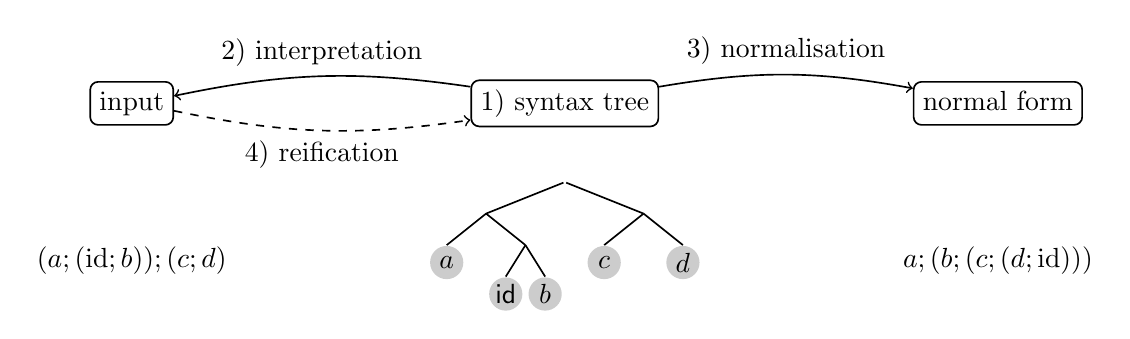
\begin{tikzpicture}[semithick]
    \begin{scope}[every node/.style = {draw, rounded corners=1mm}]
      \node (input) at  (-5.5, 2) {input\vphantom{fg}};
      \node (tree)  at  (0,    2) {1) syntax tree\vphantom{fg}};
      \node (nf)    at  (5.5,  2) {normal form\vphantom{fg}};
    \end{scope}
    \draw[->, dashed] (input) to [bend right=10] node[below] {4) reification} (tree);
    \draw[->]         (tree)  to [bend right=10] node[above] {2) interpretation} (input);
    \draw[->]         (tree)  to [bend left=10]  node[above] {3) normalisation} (nf);
    \node at (-5.5, 0) {$(a ; (\mathrm{id} ; b)) ; (c ; d)$};
    \node[inner sep=0, outer sep=0] at (0, 1) {}
      [child anchor=north,
       level/.style = {sibling distance={4cm/pow(2,#1)}, level distance=.4cm},
       every node/.style = {circle, fill=black!20, below, inner sep=-2pt, minimum width=1.2em}]
      child{
        child{node{$a$}}
        child{child{node{\textsf{id}}} child{node{$b$}}}}
      child{
        child{node{$c$}}
        child{node{$d$}}};
    \node at (5.5, 0) {$a ; (b ; (c ; (d ; \mathrm{id})))$};
  \end{tikzpicture}
  \caption{Modulo AU reasoning by reflection.}
  \label{fig:au-reflection}
\end{figure}

We carried out the metaprogramming part of the work in \RocqElpi~\cite{Tassi:habilitation}, that
lets us write \Rocq commands and tactics in \Elpi.
\Elpi is a dialect of $\lambda$Prolog, a rule-based logic programming language.
\RocqElpi has a few advantages in implementing our rewrite tactics, whose specificity is that they
may take an equation with universally quantified variables, \eg, $x$ in the hypothesis
$H : \forall x, a ; (x ; c) = f$.
Our rewrite tactics replace these variables with \emph{evars} (\emph{existential variables} or
\emph{unification variables}), \ie, unknown terms that can later be instantiated, and then, match
the pattern with evars, \eg, $a ; (\evar{x} ; c)$ where $\evar{x}$ denotes an evar, against the term
we want to rewrite to find the right instantiation for the evars.
We leverage two features of \Elpi in implementing our reification and matching procedures:
\begin{itemize}
\item When asked to reify an evar, our reification procedure \emph{suspends} by declaring
  a \emph{constraint} on the evar~\cite[Section 2.3]{Tassi:habilitation}. The constraint
  automatically \emph{resumes} when the evar get assigned by matching.
\item Our matching procedure uses \Elpi's backtracking behaviour~\cite[Section
  2.1]{Tassi:habilitation} to explore all the solutions in a brute-force manner.
  %% On the other hand, our reification procedure is checked to be fully deterministic by the recently
  %% introduced determinacy checker~\cite{FissoreTassi26}.
\end{itemize}
\pagebreak
In addition, the matching procedure of our modulo G tactics operates on AU normal forms, and
produces the witness, which can be checked by reflection, that they are equal modulo cancellation.
This design choice enables us to reuse the components of our modulo AU tactics in implementing our
modulo G tactics.

\subparagraph{Contributions}
The contributions of this paper are twofold:
\begin{enumerate}
\item\label{contrib:conciseness}
  Our modulo G tactics naturally extend the modulo AU tactics. Its implementation is sufficiently
  simple (195 LoC of \Rocq and 199 LoC of \Elpi) to allow readers to adapt it to other category
  theory libraries, and also, \emph{typed algebras}~\cite{DBLP:journals/corr/abs-1205-3612}, \ie,
  generalisations of some algebraic structures where the elements come with a source and a target.

  On the other hand, we do not aim at implementing an extension mechanism, \eg,
  \cite[Section 2]{DBLP:conf/cpp/BraibantP11} and \cite[Section 6.2]{DBLP:conf/tphol/GregoireM05},
  that allows users to declare objects to be handled by our tactics.
%% \item The reified terms for the modulo AC(U) tactics~\cite{DBLP:conf/cpp/BraibantP11} need to
%%   represent variables as identifiers, \eg, indices, so that their reflexive proof procedures can
%%   compare variables.
%%   We show that this is not the case for the modulo A(U) and G tactics. It has a consequence that
%%   handling of dependently typed terms (morphisms) becomes significantly easy.
\item\label{contrib:heterogeneity}
  We show a straightforward way to support dependently typed terms (morphisms) in the modulo
  A(U) and G tactics. In other words, we propose a solution to support one aspect of
  \emph{heterogeneity} discussed as future work by Braibant and Pous~\cite[Section
    6.2]{DBLP:conf/cpp/BraibantP11}.

  Note that our solution relies on the fact that our reified terms do not need to represent
  variables as identifiers, \eg, indices, since our normalisation procedure does not need to compare
  variables. Therefore, our solution does not extend to the modulo AC(U) tactics.
  Nonetheless, we argue that dependently-typed composition-like operators for which our solution is
  useful are non-commutative at the first place: none of the composition-like operators of typed
  algebras presented by Pous~\cite{DBLP:journals/corr/abs-1205-3612} is commutative, and the
  commutativity law does not type check for a composition-like operator of type
  $\mathrm{T}_{a, b} \to \mathrm{T}_{b, c} \to \mathrm{T}_{a, c}$.
\end{enumerate}
Thanks to Contribution \ref{contrib:conciseness}, this paper is written as a tutorial that readers
can follow to implement their own modulo AG and G tactics.
For this purpose, we recommend the \Elpi and \RocqElpi
tutorials\footnote{\url{https://github.com/LPCIC/coq-elpi\#tutorials}} as further reading.
While our actual tactics targets categories, this paper presents only their simplified versions
targeting a \emph{monoids}, \ie, categories with only one object.
This makes the type of morphisms (which are now elements of the monoid) simply typed, and simplifies
the reification and matching procedures by not carrying around type constraints.
While this choice comes with the price of obscuring Contribution \ref{contrib:heterogeneity},
we make some remarks on how the simplified version of our tactics can be generalised to the
dependently-typed case, and the implementation of our tactics for the Graph Rewriting
library is available as the supplementary material for further inspection.

\subparagraph{Outline}
The rest of this paper is organised as follows.
In \cref{sec:prelim}, we define the interfaces for monoids, and their left and/or right invertible
elements, using canonical structures~\cite{DBLP:conf/itp/MahboubiT13,rocqrefman:canonical}.
In \cref{sec:areflexivity}, we present our reflexivity modulo AU (\rocq{areflexivity}) tactic,
reified terms for reasoning modulo AU, and the reification procedure with no support for open terms,
\ie, terms with evars.
In \cref{sec:arewrite}, we present our rewriting modulo AU (\rocq{arewrite}) tactic, an extension of
the reification procedure to support open terms, and the matching modulo AU procedure.
In \cref{sec:aireflexivity}, we present our reflexivity modulo G (\rocq{aireflexivity}) tactic, a
new kind of reified terms for representing insertions and deletions of identity modulo G, \eg,
$f ; f^{-1}$, $f ; g ; g^{-1} ; f^{-1}$, and $f ; f^{-1}; g ; g^{-1}$, and the matching modulo G
procedure that explores all the possibilities of skipping an identity modulo G.
In \cref{sec:airewrite}, we present our rewrite modulo G (\rocq{airewrite}) tactic, and extend the
matching modulo G procedure to support open terms.
In \cref{sec:conclusion}, we conclude the paper.

\section{Preliminaries}
\label{sec:prelim}

In this section, we define the interfaces for monoids (\cref{sec:monoids}), and their left and/or
right invertible elements (\cref{sec:invertible}).
These structures make our tactics applicable to any monoid instance, and enables the matching
procedure to infer inverse elements.

The Graph Rewriting library defines the hierarchies of categories and morphisms~\cite[Sections 2 and
  3]{DBLP:conf/cpp/ArsacHP26} using \HB~\cite{DBLP:conf/fscd/CohenST20}, that compiles high-level
description of mathematical structures to packed classes~\cite{DBLP:conf/tphol/GarillotGMR09}.
In this paper, we \emph{neither} use \HB nor packed classes, but we use their underlying inference
mechanism called canonical structures~\cite{DBLP:conf/itp/MahboubiT13,rocqrefman:canonical}.
Our rationale is that understanding lower-level implementation details of structures, which \HB
rather obscures, is necessary for implementing our tactics, and packed classes are beneficial only
when constructing a reasonably large hierarchy with several structures and components involved,
which is not the case in our hierarchy.

While it would be feasible to reimplement our tactics for equivalent hierarchies in type
classes~\cite{DBLP:conf/tphol/SozeauO08,rocqrefman:typeclasses}, it may require a non-trivial
adaptation of the reification and matching procedures, which goes beyond the scope of this paper.

\subsection{Monoids}
\label{sec:monoids}

We define the interface for (multiplicative) monoids as follows.
\begin{rocqcode}
Module MulMonoid.
Structure type :=
  { sort : Type;
    one : sort;
    mul : sort -> sort -> sort;
    mulA : forall x y z : sort, mul x (mul y z) = mul (mul x y) z;
    mul1x : forall x : sort, mul one x = x;
    mulx1 : forall x : sort, mul x one = x; }.
End MulMonoid.
\end{rocqcode}
The record type\footnote{The \rocq{Structure} keyword is a synonym of \rocq{Record}. Following the
common convention, we use the former to distinguish the record types that are used for automatic
instance search by canonical structures.}~\cite{rocqrefman:records} above, called \rocq{type},
bundles the components of monoids: the carrier type (\rocq{sort}), the operators (\rocq{one} and
\rocq{mul}), and the non-commutative monoid laws (the rest).
This definition is surrounded by the \rocq{MulMonoid} module~\cite{rocqrefman:modules}, that acts as
a \emph{namespace}; that is, the names declared inside it are prefixed by the module name, \eg,
\rocq{MulMonoid.type}, allowing us to reuse the same internal names \rocq{type} and \rocq{sort} for
other structures.
Below, we define the shorthands for the names of the record type, operators, and monoid laws:
\begin{rocqcode}
Notation monoidType := MulMonoid.type.
Notation one := MulMonoid.one.          Notation mul := MulMonoid.mul.
Notation mulA := MulMonoid.mulA.
Notation mul1x := MulMonoid.mul1x.      Notation mulx1 := MulMonoid.mulx1.
\end{rocqcode}
declare the notations for the monoid operators:
\begin{rocqcode}
Notation "1" := one.                    Notation "x * y" := (mul x y).
\end{rocqcode}
and assume that a variable \rocq{M} always has type \rocq{monoidType}:
\begin{rocqcode}
Implicit #\PYG{k+kn}{Type}# M : monoidType.
\end{rocqcode}


Unlike type classes, the carrier type \rocq{sort}, from which we infer the monoid instance, appears
as a field of \rocq{type} rather than its parameter.
In order to use a monoid instance \rocq{M} of type \rocq{monoidType} in a context that expects its
carrier type of type \rocq{Type}, we declare the \rocq{MulMonoid.sort} projection as an implicit
coercion~\cite{rocqrefman:coercion}.
\begin{rocqcode}
Coercion MulMonoid.sort : monoidType >-> Sortclass.
\end{rocqcode}

A monoid instance can be defined as an instance of the \rocq{monoidType} record type.
In order to use it for automatic instance search by canonical structures, the instance has to be
distinguished by the \rocq{Canonical} keyword.
For example, the canonical monoid instance for lists, \ie, the free monoid, can be declared as
follows.
\begin{rocqcode}
Canonical list_monoidType (T : Type) :=
  {| MulMonoid.sort := list T;  MulMonoid.one := nil;  MulMonoid.mul := cat;
     (* Proof of the monoid laws are omitted for brevity. *) |}.
\end{rocqcode}
where \rocq{list T} is the type of lists whose elements have type \rocq{T}, \rocq{nil} is the empty
list, and \rocq{cat} is the binary concatenation operator for lists.
%
An instance search can be triggered by applying an overloaded monoid operator, \eg, \rocq{mul}, to a
term of concrete monoid type $T$, or conversely, supplying an overloaded monoid operator in a
context that expects a term of type $T$.
Type inference of such a term amounts to solving a unification problem of the form
$\text{\rocq{MulMonoid.sort}} ~ \evar{M} \unify T$ where \evar{M} is an evar representing the unknown
monoid instance for $T$, to be instantiated.
For example, if $T \coloneq \text{\rocq{list}} ~ U$, the solution is
$\evar{M} \coloneq \text{\rocq{list_monoidType}} ~ U$, because the head symbol of the
\rocq{MulMonoid.sort} field of the canonical instance \rocq{list_monoidType} is \rocq{list}.

\subsection{Invertible elements}
\label{sec:invertible}

In this section, we define four structures for invertible elements of monoids
(\cref{fig:invertible-hierarchy}).
Firstly, we define the structure that provides the common notion of inverse, but without the witness
that it is actually the inverse.
Secondly, we define the two structures of one-sided (left \emph{or} right) invertible elements, that
inherit the definition of inverse from the first structure and add the witness that it is the left
or right inverse.
Lastly, we define the structure of both-sided (left \emph{and} right) invertible elements, that
inherit the definition of inverse and its properties from the other three structures.
%% Lastly, we implement the duality between left and right inverses.
In the categorical counterpart~\cite[Section 2.2]{DBLP:conf/cpp/ArsacHP26}, the one-sided invertible
elements correspond to split monomorphisms and epimorphisms, and the both-sided invertible elements
correspond to isomorphisms.

\begin{figure}
  \centering
  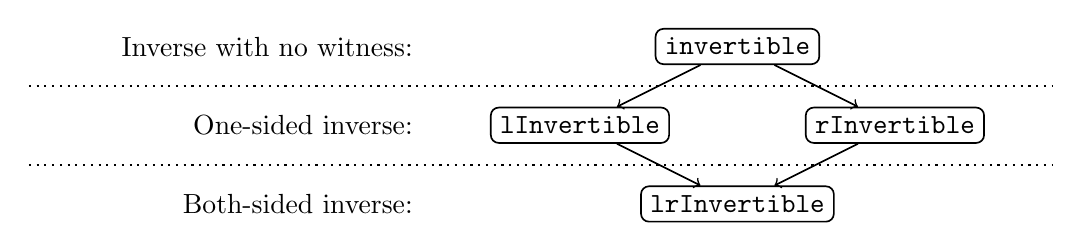
\begin{tikzpicture}
    \node[left] (zero) at (-4, 2) {Inverse with no witness:};
    \node[left] (one) at  (-4, 1) {One-sided inverse:};
    \node[left] (two) at  (-4, 0) {Both-sided inverse:};
    \begin{scope}[semithick, every node/.style = {draw, rounded corners=1mm}]
      \node (invertible)   at (0,  2) {\texttt{invertible\vphantom{I}}};
      \node (lInvertible)  at (-2, 1) {\texttt{lInvertible}};
      \node (rInvertible)  at (2,  1) {\texttt{rInvertible}};
      \node (lrInvertible) at (0,  0) {\texttt{lrInvertible}};
      \draw[->] (invertible)  to (lInvertible);
      \draw[->] (invertible)  to (rInvertible);
      \draw[->] (lInvertible) to (lrInvertible);
      \draw[->] (rInvertible) to (lrInvertible);
    \end{scope}
    \begin{scope}[thick, dotted]
      \draw (-9, 1.5) to (4, 1.5);
      \draw (-9, 0.5) to (4, 0.5);
    \end{scope}
  \end{tikzpicture}
  \caption{The hierarchy of invertible elements of monoids.}
  \label{fig:invertible-hierarchy}
\end{figure}

Given a one-sided (say, left) invertible element, its left inverses are not unique. However,
allowing to infer several left inverse elements with canonical structures is a non-trivial task.
Therefore, we assume that the inverse of any element can be \emph{canonically} determined if it
exists; that is, we can infer at most one inverse element for each element.
Our rationale of defining the first structure, that provides the unified notion of inverse for
one-sided invertible elements, is that the inverse must be unique if both left and right inverses
exist.

\subparagraph{Invertible elements with no witness}
We define the structure of invertible elements, but without the witness that the inferred invertible
element is actually the inverse.
\begin{rocqcode}
Module Invertible.
Structure type M : Type := { sort : M; inv : M; }.
End Invertible.

Notation invertible := Invertible.type.
Notation inv := Invertible.inv.
Coercion Invertible.sort : invertible >-> MulMonoid.sort.
\end{rocqcode}
where \rocq{sort} and \rocq{inv} respectively represent the invertible element and its inverse, and
\rocq{invertible} and \rocq{inv} are respectively the shorthands for the names of the record type
\rocq{Invertible.type} and the inverse constant \rocq{Invertible.inv}.

An instance search of the \rocq{invertible} structure can be triggered by a unification problem of
the form $\text{\rocq{Invertible.sort}} ~ \evar{I} \unify x$ where \evar{I} is the unknown
\rocq{invertible} instance of the given element $x$ of a monoid.

\subparagraph{Left invertible elements}
We define the structure of left invertible elements.
\begin{rocqcode}
Module LInvertible.
Structure type M : Type := { sort : M; inv : M; #\textcolor{red}{mulVx}# : inv * sort = 1; }.
End LInvertible.

Notation lInvertible := LInvertible.type.
Coercion LInvertible.sort : lInvertible >-> MulMonoid.sort.
\end{rocqcode}
Besides renaming, the only difference from the \rocq{invertible} structure above is the addition of
the new field \rocq{mulVx} to the \rocq{type} record, which says \rocq{inv} is the left inverse of
\rocq{sort}.

To implement the inheritance from \rocq{invertible} to \rocq{lInvertible}, we define the
corresponding subtyping function, as follows.
\begin{rocqcode}
(* In the \textup{LInvertible} module above *)
Definition invertible M (x : type M) :=
  {| Invertible.sort := sort x; Invertible.inv := inv x |}.
\end{rocqcode}
We declare this subtyping function as an implicit coercion from \rocq{lInvertible} instances to
\rocq{invertible} instances, and declare it as a canonical instance to solve unification problems of
the form $\text{\rocq{Invertible.sort}} ~ \evar{I} \unify \text{\rocq{LInvertible.sort}} ~ x$, as
follows.
\begin{rocqcode}
Coercion LInvertible.invertible : lInvertible >-> invertible.
Canonical LInvertible.invertible.
\end{rocqcode}

We define the shorthand \rocq{mulVx} for \rocq{LInvertible.mulVx} as follows. Note that \rocq{inv}
in the statement below comes from the \rocq{invertible} structure but not the \rocq{lInvertible}
structure, and thus, it requires the \rocq{LInvertible.invertible} coercion to typecheck.
\begin{rocqcode}
Lemma mulVx {M} (x : lInvertible M) : inv x * x = 1.
\end{rocqcode}

\subparagraph{Right invertible elements}
Symmetrically, we define the structure of right invertible elements.
\begin{rocqcode}
Module RInvertible.
Structure type M : Type := { sort : M; inv : M; mulxV : sort * inv = 1; }.
Definition invertible M (x : type M) :=
  {| Invertible.sort := sort x; Invertible.inv := inv x |}.
End RInvertible.

Notation rInvertible := RInvertible.type.
Coercion RInvertible.sort : rInvertible >-> MulMonoid.sort.
Coercion RInvertible.invertible : rInvertible >-> invertible.
Canonical RInvertible.invertible.

Lemma mulxV {M} (x : rInvertible M) : x * inv x = 1.
\end{rocqcode}

\subparagraph{Both-sided (left and right) invertible elements}
We define the structure of left \emph{and} right invertible elements, which contains all the
components of the other three structures of invertible elements.
The definitions of three subtyping functions and the declarations that they are implicit coercions
and canonical instances, that implement the inheritance from the other three structures, are omitted
for brevity.
\begin{rocqcode}
Module LRInvertible.
Structure type M : Type :=
  { sort : M; inv : M; mulVx : inv * sort = 1; mulxV : sort * inv = 1; }.
(* Define the subtyping functions here. *)
End LRInvertible.

Notation lrInvertible := LRInvertible.type.
Coercion LRInvertible.sort : lrInvertible >-> MulMonoid.sort.
(* Declare implicit coercions and canonical instances here. *)
\end{rocqcode}

%% \subparagraph{Duality}
%% We declare following canonical instances, that implement the duality between left and right
%% inverses, \ie, the fact that the inverse of left (resp.\@ right) invertible element is right
%% (resp.\@ left) invertible.
%% \begin{rocqcode}
%% Canonical inv_invertible M (x : invertible M) :=
%%   {| Invertible.sort := inv x; Invertible.inv := x |}.
%% Canonical inv_rInvertible M (x : lInvertible M) :=
%%   {| RInvertible.sort := inv x; RInvertible.mulxV := mulVx x |}.
%% Canonical inv_lInvertible M (x : rInvertible M) :=
%%   {| LInvertible.sort := inv x; LInvertible.mulVx := mulxV x |}.
%% Canonical inv_lrInvertible M (x : lrInvertible M) :=
%%   {| LRInvertible.sort := inv x;
%%      LRInvertible.mulxV := mulVx x; LRInvertible.mulVx := mulxV x |}.
%% \end{rocqcode}
%% For example, the second instance \rocq{inv_rInvertible} allows us to solve unification problems of
%% the form $\text{\rocq{RInvertible.sort}} ~ \evar{I} \unify \text{\rocq{inv}} ~ x$ given that $x$ is
%% canonically left invertible.
%% While our proof-by-reflection setup for the tactics modulo G
%% (\cref{sec:aireflexivity,sec:airewrite}) directly supports only right-invertible elements, our
%% modulo G tactics also support left-invertible elements through duality.

\section{Reflexivity modulo AU}
\label{sec:areflexivity}

\subparagraph{Reflection}
In this section, we implement the reflexivity modulo AU (\rocq{areflexivity}) tactic.
To this end, we define our proof-by-reflection setup depicted in \cref{fig:au-reflection}.
We first define reified syntax trees as the following inductive datatype:
\begin{rocqcode}
Inductive aexpr M : Type :=
  ae_mul : aexpr M -> aexpr M -> aexpr M | ae_one : aexpr M | ae_var : M -> aexpr M.
\end{rocqcode}
whose three constructors respectively represent the monoid operators \rocq{mul} and \rocq{one}, and
a variable, \ie, any element of the monoid \rocq{M}.
Any syntax tree can be interpreted and put in its right-leaning normal form respectively by the
following functions \rocq{ae_eval} and \rocq{ae_norm}.
\begin{rocqcode}
Fixpoint ae_eval {M} (e : aexpr M) : M :=
  match e with
  | ae_mul e1 e2 => ae_eval e1 * ae_eval e2 | ae_one => 1 | ae_var x => x
  end.

Fixpoint ae_norm {M} (e : aexpr M) (acc : M) : M :=
  match e with
  | ae_mul e1 e2 => ae_norm e1 (ae_norm e2 acc)
  | ae_one => acc | ae_var x => x * acc
  end.
\end{rocqcode}
The latter function takes an accumulator \rocq{acc} in addition to a syntax tree \rocq{e}, and
computes the normal form of \rocq{ae_eval e * acc}, \ie, \rocq{(x1 * (..(xn * acc)..))} given that
\rocq{e} represents \rocq{x1 * .. * xn} modulo AU.
Thus, $\phi(e)$ and $\mathsf{norm}(e)$ in \cref{sec:introduction} correspond to \rocq{ae_eval e}
and \rocq{ae_norm e 1}, respectively.
Then, \cref{prop:ae_correct,prop:areflexivity_correct} can be proved in \Rocq as the following
lemmas.
\begin{rocqcode}
Lemma ae_correct {M} (e : aexpr M) (acc : M) : ae_eval e * acc = ae_norm e acc.
Proof. (* By structural induction on \textup{e}. *) Qed.

Lemma areflexivity_correct {M} (e1 e2 : aexpr M) :
  ae_norm e1 1 = ae_norm e2 1 -> ae_eval e1 = ae_eval e2.
\end{rocqcode}

Suppose we want to prove a goal \rocq{(x * y) * z = x * (y * z)} for some elements \rocq{x},
\rocq{y}, and \rocq{z} of a monoid \rocq{M}.
Thanks to the above reflection lemma, the proof can be done by the following proof term:
\begin{rocqcode}
let e1 := ae_mul (ae_mul (ae_var x) (ae_var y)) (ae_var z) in
let e2 := ae_mul (ae_var x) (ae_mul (ae_var y) (ae_var z)) in
@areflexivity_correct M e1 e2 erefl
\end{rocqcode}
where \rocq{e1} and \rocq{e2} are reified terms of the LHS and RHS, respectively.
To type-check this proof term, we use computational reflection twice.
Firstly, applying the above term to the given goal requires \rocq{ae_eval e1 = ae_eval e2} and the
goal to be convertible.
Secondly, supplying \rocq{erefl}, the reflexivity of the equality \rocq{=}, as the proof of
\rocq{ae_norm e1 1 = ae_norm e2 1} requires \rocq{ae_norm e1 1} and \rocq{ae_norm e2 1} to be
convertible.

\subparagraph{Reification}
The missing piece for implementing the \rocq{areflexivity} tactics is the \emph{reification}
procedure that performs the inverse of the interpretation function \rocq{ae_eval}.
It can be implemented in \RocqElpi~\cite{Tassi:habilitation} (\cref{sec:introduction}) as follows.
\begin{elpicode}
pred quote i:term i:term o:term. #\label{line:quote}#
quote M {{ @one lp:M' }} {{ @ae_one lp:M }} :- coq.unify-eq M M' ok, !. #\label{line:quote:one}#
quote M {{ @mul lp:M' lp:In1 lp:In2 }} {{ @ae_mul lp:M lp:Out1 lp:Out2 }} :- #\label{line:quote:mul}#
  coq.unify-eq M M' ok, !, quote M In1 Out1, quote M In2 Out2.
quote M In {{ @ae_var lp:M lp:In }} :- !. #\label{line:quote:var}#
\end{elpicode}
Line \ref{line:quote} declares that \elpi{quote} is a \emph{predicate} with three parameters of type
\elpi{term}, which is the type of \Rocq terms embedded in \Elpi; in other words, \elpi{quote} is a
relation between three \Rocq terms.
These parameters are respectively a monoid \elpi{M}, a monoid expression \elpi{In} of type \elpi{M},
and the reified term \elpi{Out} of \elpi{In}.
Since our objective is to calculate the reified term given the other parameters, we mark the first
two parameters as the \emph{input} (\texttt{i:}) and the last one as the \emph{output}
(\texttt{o:}).

The rest of the code gives three \emph{rules} that specifies the behaviour of \elpi{quote}.
The syntax \elpi|{{ ... }}| is the \emph{quotation} that lets us write \Rocq terms embedded in \Elpi
using the syntax of \Rocq, and conversely, \rocq{lp:} is the antiquotation that lets us use \Elpi
syntax in the quoted \Rocq terms~\cite[Section 3.4.1]{Tassi:habilitation}.
%
The first rule (Line \ref{line:quote:one}) reifies \rocq{one} to \rocq{ae_one M}.
The second rule (Line \ref{line:quote:mul}) reifies \rocq{mul} to \rocq{@ae_mul M}, and also,
recursively reifies the arguments \elpi{In1} and \elpi{In2} of \rocq{mul} to \elpi{Out1} to
\elpi{Out2}, respectively, by calling \rocq{quote} itself.
The last rule (Line \ref{line:quote:var}) handles the variables by reifying the other terms to
\rocq{@ae_var M}.

The first two rules follow the \emph{reification by small-scale reflection}
approach~\cite[Section 3.2]{DBLP:conf/itp/Sakaguchi22}; that is, we compare the two monoid instances
\elpi{M} and \elpi{M'}, respectively given as the first argument of \elpi{quote} and the implicit
argument of the monoid operator (\rocq{one} or \rocq{mul}), by conversion. The conversion checking
is done by calling the unification API of \Rocq (\elpi{coq.unify-eq}).
This approach allows us to rule out the case where \elpi{M} and \elpi{M'} are not the same monoid,
while supporting the case where they are syntactically unequal but still convertible.
Such monoid instances may exist in the presence of structures that inherit from monoids, \eg, groups
and rings~\cite{DBLP:conf/cade/AffeldtCKMRS20}.
The case where \elpi{M} and \elpi{M'} are inconvertible are handled by the last rule thanks to the
backtracking.

Backtracking in \Elpi can be controlled by the cut operator (\elpi{!}), that commits to the
currently chosen rule by discarding the other rules.
In the first two rules, the cut is placed after \elpi{coq.unify-eq} since we want to backtrack when
the conversion fails; that is, this conversion is considered to be a part of the pattern matching.
Thanks to the cut operator, \elpi{quote} is \emph{deterministic}; that is, it returns at most one
solution for each invocation.
Replacing Line \ref{line:quote} with the following signature instructs the determinacy
checker~\cite{FissoreTassi26} to check this property.
\begin{elpicode}
func quote term, term -> term.
\end{elpicode}

\subparagraph{The tactic}
The \rocq{areflexivity} tactic can be implemented as the following rule of the \elpi{solve}
predicate, which is the entry point for tactics in \RocqElpi.
\begin{elpicode}
solve (goal _ _ Type _ _ as G) [] :- !,
  coq.unify-eq Type {{ @eq (MulMonoid.sort lp:M) lp:LHS lp:RHS }} ok, #\label{line:areflexivity:unif}#
  quote M LHS LHSQ, quote M RHS RHSQ, #\label{line:areflexivity:quote}#
  refine {{ @areflexivity_correct lp:M lp:LHSQ lp:RHSQ erefl }} G [].  #\label{line:areflexivity:refine}#
\end{elpicode}
where \elpi{solve G GS} means that the tactic takes a goal \elpi{G} and returns a list of subgoals
\rocq{GS}. We use the empty list \elpi{[]} as \elpi{GS} since our tactic should not leave any
subgoal, \ie, either completely solve the given goal \elpi{G} or fail.
Line \ref{line:areflexivity:unif} asserts that the goal is an equation over monoid. It does so by
unifying the goal with \rocq{@eq (MulMonoid.sort #$\evar{M}$#) #$\evar{LHS}$# #$\evar{RHS}$#}.
Line \ref{line:areflexivity:quote} reifies the \elpi{LHS} and \elpi{RHS} to \elpi{LHSQ} and
\elpi{RHSQ}, respectively.
Line \ref{line:areflexivity:refine} attempts to close the goal \elpi{G} using the proof term
\rocq{areflexivity_correct M LHSQ RHSQ erefl}.

\subparagraph{Dependently-typed case}
In order to generalise the \rocq{areflexivity} tactic to morphisms in a category, \rocq{aexpr}
should be defined as an inductive family that takes the source and target objects as parameters.
Its interpretation and normalisation procedures, and the lemmas should be adapted accordingly.
The adaptation of \rocq{ae_norm} to such a datatype requires the \emph{convoy pattern} to typecheck;
that is, the \rocq{match} expression should return a function that takes \rocq{acc}.
In this case, our \elpi{quote} predicate takes the source and target objects of the input \elpi{In},
since we need them for constructing the output \elpi{Out}, and we avoid inferring them from the
input for performance reasons.

\section{Rewriting modulo AU}
\label{sec:arewrite}

In this section, we implement the rewriting modulo AU (\rocq{arewrite}) tactic, which behaves as
follows:
\begin{enumerate}
\item It takes a subterm \rocq{e} of the goal and a proof of an equation \rocq{lhs = rhs}.
  While \rocq{e} must be a ground term, the equation may be universally quantified and may include
  side conditions.
\item It instantiates the quantifiers and side conditions of the given proof with evars.
\item It finds \rocq{pre} and \rocq{post} such that \rocq{pre * lhs * post} is equal to \rocq{e};
  that is, it matches the pattern \rocq{#$\evar{pre}$# * lhs * #$\evar{post}$#} against \rocq{e}
  modulo AU.
\item It rewrites \rocq{e} in the goal to \rocq{pre * rhs * post}.
\end{enumerate}
While we reuse our proof-by-reflection setup (\cref{sec:areflexivity}), we introduce a new
reflection lemma:
\begin{rocqcode}
Lemma arewrite_correct {M} (e lhs : aexpr M) (rhs : M) :
  ae_norm e 1 = ae_norm lhs 1 -> ae_eval lhs = rhs -> ae_eval e = rhs.
\end{rocqcode}
where \rocq{lhs} and \rocq{rhs} are already expanded with \rocq{pre} and \rocq{post}.
While the first hypothesis (\rocq{ae_norm e 1 = ae_norm lhs 1}) should be proved by reflection, the
second one (\rocq{ae_eval lhs = rhs}) corresponds to the equation supplied by the user.

In the rest of this section, we adapt the \elpi{quote} predicate to rewriting modulo AU and
implement the matching modulo AU procedure.

\subparagraph{Reification}
The adaptation of the \elpi{quote} predicate is twofold:
\begin{itemize}
\item adding the support for open terms, \ie, the presence of evars in the input, and
\item flattening the input into a list-like structure, which we call \emph{paths}, to be used by the
  matching procedure.
\end{itemize}
We first define paths as a datatype in \Elpi as follows:
\begin{elpicode}
kind path type.
type nilp path.
type consp term -> path -> path.
type catp path -> path -> path.
\end{elpicode}
where \elpi{path} is the name of the datatype, \elpi{nilp} is the constructor representing
\rocq{one}, \elpi{consp} is the constructor representing a multiplication (\rocq{mul}) of a variable
and a path, and \elpi{catp} is another constructor representing a multiplication, but whose LHS must
be an evar.

We modify the \elpi{quote} predicate to produce the path as follows:
\begin{elpicode}
func quote term, term -> term, path.
quote M In Out (OutP nilp) :- !, quote-rec M In Out OutP.

func quote-rec term, term -> term, (path -> path).
quote-rec M {{ @one lp:M' }} {{ @ae_one lp:M }} (p\ p) :- coq.unify-eq M M' ok, !.
quote-rec M {{ @mul lp:M' lp:In1 lp:In2 }}
    {{ @ae_mul lp:M lp:Out1 lp:Out2 }} (p\ OutP1 (OutP2 p)) :-
  coq.unify-eq M M' ok, !, quote-rec M In1 Out1 OutP1, quote-rec M In2 Out2 OutP2.
quote-rec M In {{ @ae_var lp:M lp:In }} (consp In).
\end{elpicode}
where the syntax \elpi{(x\ e)} represents a function, \ie, $(\lambda x. e)$.
To avoid linear-time concatenation of paths, the \elpi{quote-rec} predicate produces a path in the
form of \emph{difference lists}, \ie, a function of type \elpi{path -> path} that prepends the path
it represents to the given path.

We further extend the \elpi{quote-rec} predicate to support open terms, by adding the rule below
\emph{as the first rule} of \elpi{quote-rec}:
\begin{elpicode}
quote-rec M In Out (catp OutP) :-
  var In, !, declare_constraint (path.quote M OutP In Out) OutP.
\end{elpicode}
where \elpi{var In} asserts that \elpi{In} is a \emph{unification variable}, \ie, representing an
evar in \Rocq.
In this case, we \emph{suspend} the reification process: \elpi{declare_constraint C V} declares the
constraint \elpi{C} on the unification variable \elpi{V}, which means that \elpi{C} resumes upon the
assignment of \elpi{V}.
Note that we declare the constraint not on the input \elpi{In}, but on the path \elpi{OutP}.
This is because our matching procedure operates on paths and instantiates unification variables in
them, and we need to change the roles of input and output here.
The constraint \elpi{path.quote M OutP In Out}, defined below, is a version of the reification
procedure that takes the path \elpi{OutP} as the input and produces the input and the reified term.
\begin{elpicode}
func path.quote term, path -> term, term.
path.quote M P Out OutQ :- var P, !, declare_constraint (path.quote M P Out OutQ) P.
path.quote M nilp {{ @one lp:M }} {{ @ae_one lp:M }} :- !.
path.quote M (consp _ P' as P) Out OutQ :-
  var P', !, declare_constraint (path.quote M P Out OutQ) P'.
path.quote M (consp X nilp) X {{ @ae_var lp:M lp:X }} :- !.
path.quote M (consp X P)
    {{ @mul lp:M lp:X lp:Out }} {{ @ae_cons lp:M lp:X lp:OutQ }} :-
  path.quote M P Out OutQ.
\end{elpicode}
The \elpi{path.quote} predicate does not need to support \elpi{catp} since our matching procedure
does not produce it, and can suspend and resume again when the given path is either a unification
variable or \elpi{consp X P} where \elpi{P} is a unification variable.

\subparagraph{Matching}
We define our matching procedure as follows:
\begin{elpicode}
pred path.match i:path, o:path.
path.match nilp nilp :- !.
path.match (consp X P) (consp X' P') :- !, coq.unify-eq X X' ok, path.match P P'.
path.match P (catp Pl' Pr') :- path.split P Pl Pr, Pl' = Pl, path.match Pr Pr'.
\end{elpicode}
where \elpi{path.match P P'} matches the path (pattern) \elpi{P'} against the path \elpi{P}, and only
\elpi{P'} may contain evars.
The first two rules handle \elpi{nilp} and \elpi{consp} in a pointwise manner.
The last rule handles the case where \elpi{P'} is \elpi{catp Pl' Pr'} for some evar \elpi{Pl'}.
It proceeds by splitting \elpi{P} into a left part \elpi{Pl} and the rest \elpi{Pr}, instantiating
\elpi{Pl'} with \elpi{Pl} (thus resuming the constraint declared on \elpi{Pl'}), and matching
\elpi{Pr'} against \elpi{Pr}.
The splitting procedure \elpi{path.split} is defined as follows:
\begin{elpicode}
pred path.split i:path, o:path, o:path.
path.split P nilp P.
path.split (consp X P) (consp X Pl) Pr :- path.split P Pl Pr.
\end{elpicode}
Note that these predicates relies on backtracking and are nondeterministic:
\elpi{path.split} returns all the solutions from left to right in terms of the point that splits the
given path, and \elpi{path.match} explores all the possibilities of instantiating evars.

\subparagraph{Dependently-typed case}
As we described in \cref{sec:areflexivity}, we need to carry around some source and target objects
of the morphisms we handle in the dependently-typed case.
For example, we chose to add the object in the middle of the composition to the \elpi{consp} and
\elpi{catp} constructors, and extend the \elpi{quote}, \elpi{quote-rec}, and \elpi{path.quote}
predicates with the source and target objects of their input.
Most notably, the second rule of \elpi{path.match} should split the path \elpi{P} at the target
object of \elpi{Pl'}, and thus, we extended \elpi{path.split} with the object that splits the given
path. This change prunes the search space of the matching.

In addition, the Graph Rewriting library generalises the morphism equality from Leibniz equality
(\rocq{eq}) to setoid equalities~\cite[Section 2.1]{DBLP:conf/cpp/ArsacHP26}. Nevertheless, adapting
our tactics to setoid equalities is just a matter of adapting our reflection lemmas and discharging
the task of inferring a setoid morphism to the standard \rocq{setoid_rewrite} tactic.

\section{Reflexivity modulo G}
\label{sec:aireflexivity}

In this section, we implement the reflexivity modulo G (\rocq{aireflexivity}) tactic.
Firstly, we implement another layer of reflection that deals only with cancellation, to be combined
with the reflection setup from \cref{sec:areflexivity}.
This separation between associativity and cancellation allows us to use the reification procedure
from \cref{sec:areflexivity,sec:arewrite} as is.
Secondly, we implement a matching modulo G procedure, which we extend to support open terms in
\cref{sec:airewrite}.

\subparagraph{Reflection}
We argue that reasoning modulo cancellation amounts to inserting and deleting sequences described by
$I$ in the following grammar:
\begin{align*}
  I &\coloneq x \, I^* \, x^{-1} & \text{($x$ is right invertible, \ie, $x \times x^{-1} = 1$)} \\
  I^* &\coloneq 1 \mid I \, I^*  & \text{(The Kleene star on $I$)}
\end{align*}
and such insertions and deletions can always be done with no overlap.\todo{Proof?}
We define the reified syntax for $I$ as a version of rose trees:
\begin{rocqcode}
Inductive iexpr M : Type := can_inv : rInvertible M -> list (iexpr M) -> iexpr M.
\end{rocqcode}
and its interpretation
$\phi_I(\text{\rocq{can_inv}} ~ x ~ [e_1, \dots, e_n])
  \coloneq x \, \phi_I(e_1) \dots \phi_I(e_n) \, x^{-1}$
in the \emph{right-leaning normal form} as follows:
\begin{rocqcode}
Fixpoint ie_eval {M} (e : iexpr M) (acc : M) : M :=
  let: can_inv x es := e in x * foldr ie_eval (inv x * acc) es.
\end{rocqcode}
We define another reified syntax for sequences with insertions and deletions of $I$:
\begin{rocqcode}
Inductive cexpr M : Type :=
  | ce_cons : M -> cexpr M -> cexpr M | ce_one : cexpr M
  | ce_icons (f : bool) : iexpr M -> cexpr M -> cexpr M.
\end{rocqcode}
where \rocq{ce_icons} represents an insertion or deletion of $I$, depending on whether \rocq{f} is
\rocq{true} or \rocq{false}.
We define its interpretation, again in the right-leaning normal form, as follows:
\begin{rocqcode}
Fixpoint ce_eval {M} (f : bool) (e : cexpr M) (acc : M) : M :=
  match e with
  | ce_cons m e => m * ce_eval f e acc | ce_one => acc
  | ce_icons f' e1 e2 => (if eqb f f' then ie_eval e1 else id) (ce_eval f e2 acc)
  end.
\end{rocqcode}
where \rocq{ce_eval f} interprets the \rocq{ce_icons f'} constructor only if \rocq{f = f'} and
discards it otherwise.
Therefore, flipping the Boolean value \rocq{f} flips the insertions and deletions of $I$ represented
by \rocq{ce_icons}, which is justified by the following lemma:
\begin{rocqcode}
Lemma ce_correct {M} (e : cexpr M) acc : ce_eval false e acc = ce_eval true e acc.
\end{rocqcode}
To prove that the given two monoid expressions are equal modulo G, we prove the following reflection
lemma, which combines the new definitions above with the reflection setup for our modulo AU tactics
(\cref{sec:areflexivity}):
\begin{rocqcode}
Lemma aireflexivity_correct {M} (e1 e2 : aexpr M) (ce : cexpr M) :
  ae_norm e1 1 = ce_eval false ce 1 -> ce_eval true ce 1 = ae_norm e2 1 ->
  ae_eval e1 = ae_eval e2.
\end{rocqcode}
where \rocq{e1} and \rocq{e2} are reified syntax trees of the given expressions for reasoning modulo
AU, and \rocq{ce} justifies the fact that the normal forms of \rocq{e1} and \rocq{e2} can be equated
by insertions and deletions of $I$.

\subparagraph{Matching}
The matching modulo G procedure needs to explore all the possibilities of skipping $I$ in the given
paths to find a solution.
Firstly, we define a utility predicate \elpi{rinv->linv M X Ri RV} that infers right invertibility
of \elpi{X} of type \elpi{M} and returns its \rocq{rInvertible} instance \elpi{Ri}
(\cref{sec:invertible}) and its right inverse \elpi{RV}:
\begin{elpicode}
func rinv->linv term, term -> term, term.
rinv->linv M X {{ @inv_rInvertible lp:M lp:Li }}
               {{ @LInvertible.sort lp:M lp:Li }} :-
  coq.unify-eq X {{ @inv lp:M (@LInvertible.invertible lp:M lp:Li) }} ok, !.
rinv->linv M X Ri {{ @inv lp:M (@RInvertible.invertible lp:M lp:Ri) }} :-
  coq.unify-eq X {{ @RInvertible.sort lp:M lp:Ri }} ok, !.
\end{elpicode}
where
\rocq{inv_rInvertible} turns a given \rocq{lInvertible} instance into the \rocq{rInvertible}
instance on its inverse,
the first rule applies when \elpi{X} unifies with \rocq{inv Y} for some left invertible
\rocq{Y}, and
the second rule triggers canonical structure inference by unification:
$\text{\rocq{RInvertible.sort}} ~ \evar{Ri} \unify \text{\elpi{X}}$.

Secondly, we define two predicates for recognising a prefix of the form $I$ and $I^*$, respectively.
The first predicate \elpi{skip-one M P P' Out} splits a given path \elpi{P} into a prefix of the
form $I$ and the rest of the path \elpi{P'}, and reify the former to \elpi{Out} of type
\rocq{iexpr M}.
The second predicate \elpi{skip-ones M P P' Out} does the same for $I^*$, where \elpi{Out} is a list
of reified terms of type \rocq{iexpr M}.
We define them via mutual recursion as follows:
\begin{elpicode}
func skip-one term, path -> path, term.
skip-one M (consp X P) P' {{ @can_inv lp:M lp:Ri lp:Out }} :- !,
  rinv->linv M X Ri XV, !,              % check if \textup{X} is right invertible
  skip-ones M P (consp XV' P') OutL,    % skip $I^*$
  coq.unify-eq XV XV' ok,               % check if \textup{XV'} is the inverse of \textup{X}
  !, % commit to the first solution
  mkrocqlist {{ @iexpr lp:M }} OutL Out.% turns a list in \Elpi into a list in \Rocq

pred skip-ones i:term, i:path, o:path, o:list term.
skip-ones _ P P [].
skip-ones M P P2 [Out1|Out2] :- skip-one M P P1 Out1, !, skip-ones M P1 P2 Out2.
\end{elpicode}
Note that \elpi{skip-ones} uses backtracking to enumerate the solutions from shorter ones to longer
ones, \ie, $I^0$, $I$, $I^2$, and so on.
A path may have several prefixes of the form $I$; for example, both $(x (x^{-1} x) x^{-1})$ and its
prefix $(x x^{-1})$, where $x^{-1}$ is the both-sided inverse of $x$, are of the form $I$.
Given such a path, \elpi{skip-one} commits to the first (shortest) solution using the cut operator
\elpi{!}.
This avoids duplicated or missing solutions in the enumeration by \elpi{skip-ones} because, if a
path has several prefixes of the form $I$, such an ambiguity is always introduced by the presence of
a both-sided inverse, and we can always reach to later solutions by repetitively taking the shortest
prefix, \eg, $(x x^{-1}) (x x^{-1})$.

Lastly, we implement the matching modulo G procedure as two predicates \elpi{path.match} and
\elpi{path.match'}. Both of them take four parameters \elpi{M}, \elpi{P}, \elpi{Q}, and \elpi{Out},
attempt to match the two paths \elpi{P} and \elpi{Q}, and produce the witness \elpi{Out} of type
\rocq{cexpr M} that \elpi{P} and \elpi{Q} are equal modulo cancellation.
The former skips a prefix of the form $I^*$ of each path, the latter skip the first item of each
path given that they are the same, and they call each other to match the rest of the paths.
Therefore, we define them via mutual recursion as follows:
\begin{elpicode}
pred path.match i:term, i:path, i:path, o:term.
path.match M P Q Out'' :-
  skip-ones M P P' OutP,
  skip-ones M Q Q' OutQ,
  path.match' M P' Q' Out,
  iexprs->cexpr M {{ false }} OutP Out Out',
  iexprs->cexpr M {{ true }} OutQ Out' Out''.

pred path.match' i:term, i:path, i:path, o:term.
path.match' M nilp nilp {{ @ce_one lp:M }} :- !.
path.match' M (consp X P) (consp X' Q) {{ @ce_cons lp:M lp:X lp:Out }} :- !,
  coq.unify-eq X X' ok, path.match M P Q Out.
\end{elpicode}
where \elpi{iexprs->cexpr M F IES CE Out} prepends a list \elpi{IES} of terms of type \rocq{iexpr M}
to a term \elpi{CE} of type \rocq{cexpr M} by the constructor \rocq{ce_icons F}.

\section{Rewriting modulo G}
\label{sec:airewrite}

In this section, we implement the rewriting modulo G (\rocq{airewrite}) tactic.
We first introduce the following reflection lemma:
\begin{rocqcode}
Lemma airewrite_correct {M} (e lhs : aexpr M) (rhs : M) (ce : cexpr M) :
  ae_norm e 1 = ce_eval false ce 1 -> ce_eval true ce 1 = ae_norm lhs 1 ->
  ae_eval lhs = rhs -> ae_eval e = rhs.
\end{rocqcode}
where \rocq{e} represents the subterm of the goal to be rewritten, \rocq{lhs} and \rocq{rhs}
represent the LHS and RHS of the equation expanded with \rocq{pre} and \rocq{post}
(\cref{sec:arewrite}), and \rocq{ce} is the witness that \rocq{e} and \rocq{lhs} are equal modulo G.

\subparagraph{Matching}
In the rest of this section, we extend the matching modulo G procedure (\cref{sec:aireflexivity})
with the support for open terms.
Firstly, we modify the \elpi{skip-one} and \elpi{skip-ones} predicates, which respectively finds a
prefix of the form $I$ and $I^*$ of the given path, as follows:
\begin{elpicode}
pred skip-one i:term, o:path, o:path, o:term.
skip-one M (consp X P) P'' {{ @can_inv lp:M lp:Ri lp:Out }} :- !,
  rinv->linv M X Ri XV, !,
  skip-ones M P P' OutL,
  ((P' = consp XV' P'', !, coq.unify-eq XV XV' ok);
   (P' = catp (consp XV Pl) Pr, !, P'' = catp Pl Pr)),
  !,
  mkrocqlist {{ @iexpr lp:M }} OutL Out.

pred skip-ones i:term, o:path, o:path, o:list term.
% The rules of \textup{skip-ones} remain unchanged, and are omitted for brevity.
\end{elpicode}
where \elpi{;} is the disjunction operator: \elpi{P; Q} first attempts \elpi{P} and then \elpi{Q}.
The changes from \cref{sec:aireflexivity} are twofold:
\begin{itemize}
\item These predicates may now instantiate the given path, \ie, their second argument, where
  unification variables always appear as the first argument of \elpi{catp}.
  Therefore, these parameters are marked as output (\texttt{o:}), and \elpi{skip-one} is not
  deterministic anymore.
\item In the rule of \elpi{skip-one}, if the path \elpi{P'} (the output of \elpi{skip-ones}) starts
  with a unification variable, we close the ``open parenthesis'', \ie, the right invertible element
  \elpi{X}, by instantiating the head of the unification variable with its inverse \elpi{XV}.
  Since \elpi{skip-one} recursively calls itself, it can recursively close several open parentheses;
  that is, it can split a path of the form $x_1 \, I^* \dots x_n \, I^* \, \evar{P}$, where
  $x_1, \dots, x_n$ are right invertible, into $x_1 \, I^* \dots x_n \, I^* x_n^{-1} \dots x_1^{-1}$
  and the rest, by instantiating $\evar{P}$ with $x_n^{-1} \dots x_1^{-1} \, \evar{P'}$.
\end{itemize}
Note that our solution is not the only way of ``closing the parentheses'' since we may find a part
of $x_n^{-1} \dots x_1^{-1}$ after the unification variable.
For example, $x \, y \, \evar{P} \, x^{-1}$ is of the form $I$ if we instantiate $\evar{P}$ with
$g^{-1}$.
Nevertheless, we argue that it is safe to immediately close the parentheses, \ie, instantiate
$\evar{P}$ with $y^{-1} \, x^{-1} \, \evar{P'}$, since we can then open the parentheses again, \ie,
instantiate $\evar{P'}$ with $x$.
To sum up, our solution to the above example $x \, y \, \evar{P} \, x^{-1}$ is to instantiate
$\evar{P}$ with $y^{-1} \, x^{-1} \, x$, which results in
$(x \, y \, y^{-1} \, x^{-1}) \, (x \, x^{-1})$.
However, our solution may not work if the unification variable $\evar{P}$ appear more than once in
the path.
We intentionally leave such cases \emph{unsupported}, since multiple occurrences of the same
unification variable correspond to a cycle in a diagram, which are uncommon in typical categorical
reasoning.

Secondly, we modify the matching modulo G procedure, the \elpi{path.match} and \elpi{path.match'}
predicates.
We change their signatures, for the same reason as above:
\begin{elpicode}
pred path.match i:term, i:path, o:path, o:term.
pred path.match' i:term, i:path, o:path, o:term.
\end{elpicode}
While their rules remain unchanged from \cref{sec:aireflexivity}, we add the following new rule of
\elpi{path.match'}:
\begin{elpicode}
path.match' M P (catp QVar Q) Out'' :-
  skip-one_catp M Q [] Qr QlV QlW,
  path.split P Pl Pr,
  path.cat Pl QlV QVar,
  path.match M Pr Qr Out,
  iexprs->cexpr M {{ true }} QlW Out Out',
  path->cexpr M Pl Out' Out''.
\end{elpicode}
This rule matches a pattern \elpi{catp QVar Q}, where \elpi{QVar} is a unification variable, against
a path \elpi{P}. It consists of the following two steps:
\begin{itemize}
\item The \elpi{skip-one_catp} predicate performs the dual operation of ``closing the parentheses'';
  that is, it splits the given path \elpi{Q} into a prefix of the form $I^* \, x_1 \dots I^* \, x_n$
  and the rest \elpi{Qr}, where $x_1, \dots, x_n$ are \emph{left} invertible.
  It also produces a path \elpi{QlV}, which is $x_n^{-1} \dots x_1^{-1}$, and a witness \elpi{QlW}
  that the concatenation of \elpi{QlV} and the prefix, \ie,
  $x_n^{-1} \dots x_1^{-1} \, I^* \, x_1 \dots I^* \, x_n$, is of the form $I^*$.

  Note that the only case where this sequence is \emph{not} of the form $I$ is when the prefix is
  empty. Therefore, the witness \elpi{QlW} is \emph{not} a term of type \rocq{iexpr M}, but a list
  of terms of type \rocq{iexpr M}, which is either empty or singleton.
\item As in the matching modulo AU procedure (\cref{sec:arewrite}), \elpi{path.split} splits
  \elpi{P} into \elpi{Pl} and \elpi{Pr}.
  We then instantiate the unification variable \elpi{QVar} with the concatenation of \elpi{Pl} and
  \elpi{QlV}, obtained by \elpi{path.cat}, and match the rest of the pattern \elpi{Qr} against
  \elpi{Pr}.
\end{itemize}
Again, backtracking is at the core of the matching procedure: both \elpi{skip-one_catp} and
\elpi{path.split} explore all the solutions, from left to right in terms of the point that splits
the given path.
To build the witness, the \elpi{path->cexpr} predicate prepends the path \elpi{Pl} to
the witness of type \elpi{cexpr M}.

Lastly, the \elpi{skip-one_catp} predicate is defined as follows:
\begin{elpicode}
pred skip-one_catp i:term, i:path, i:list term, o:path, o:path, o:list term.
skip-one_catp _ P Acc P nilp Acc.
skip-one_catp M P Acc Q (consp EV PV) Acc'''' :-
  skip-ones M P (consp E P') Acc',
  linv->rinv M E Ri EV,
  std.append Acc Acc' Acc'', % appends two lists \textup{Acc} and \textup{Acc'} into \textup{Acc''}
  mkrocqlist {{ @iexpr lp:M }} Acc'' Acc''',
  skip-one_catp M P' [{{ @can_inv lp:M lp:Ri lp:Acc''' }}] Q PV Acc''''.
\end{elpicode}
where \elpi{linv->rinv} performs the dual of \elpi{rinv->linv}; that is, it takes a left invertible
element \elpi{E}, and returns its inverse \elpi{EV} and a right invertible instance \elpi{Ri} on
\elpi{EV}.

\section{Conclusion}
\label{sec:conclusion}

We presented tactics for equational reasoning modulo AU (associativity and unit) and G (AU and
inverse) in \Rocq.
We implemented two versions of the tactics, and both of them are available in the supplementary
material:
1) simply-typed versions presented in the paper, and
2) dependently-typed versions for category theory, built on top of the Graph Rewriting
library~\cite{DBLP:conf/cpp/ArsacHP26}.
The dependently-typed versions of the tactics consist of 195 LoC of \Rocq and 199 LoC of \Elpi,
excluding the code from the Graph Rewriting library.
We argue that the implementation of our tactics is sufficiently simple to allow readers to adapt it
to other category theory libraries.
Moreover, the present work illustrates a broader shift in ITP, that the development of advanced
automation tools, which used to require expert knowledge, \eg, writing a \Rocq plugin in \OCaml, is
now a lot more accessible to end users thanks to recent technologies, \eg, \RocqElpi.
This is one of the reasons why we chose \emph{not} to provide an extension mechanism for declaring
objects to be handled by our tactics, \eg, \cite[Section 2]{DBLP:conf/cpp/BraibantP11} and
\cite[Section 6.2]{DBLP:conf/tphol/GregoireM05}.

We believe that the following factors largely contributed to the simplicity and conciseness of the
implementation of our tactics:
\begin{description}
\item[Avoiding identifiers and variable maps]
  Typical reflexive tactics, \eg, \cite{DBLP:conf/cpp/BraibantP11,DBLP:conf/tphol/GregoireM05}, use
  reified syntax trees whose leaves are replaced by identifiers that the proof procedure can
  compare. Interpreting such syntax trees requires a so-called \emph{variable map}, that maps
  identifiers to their corresponding term. The presence of these identifiers and variable maps make
  handling of heterogeneous, \eg, dependently-typed, syntax trees cumbersome. Therefore,
  it was crucial to observe that we can perform modulo AU and G reasoning without them.
\item[The modular design of the proof-by-reflection setup]
  Our modulo G tactics (\cref{sec:aireflexivity,sec:airewrite}) use proof by reflection twice: once
  for modulo AU reasoning, and once more for modulo cancellation reasoning, of which the former is
  shared with our modulo AU tactics (\cref{sec:areflexivity,sec:arewrite}).
  While our approach may have a slight performance disadvantage over designing a reified syntax that
  deals with modulo G reasoning at once, our approach allowed us to reuse the concept of paths and
  the reification procedure (\cref{sec:arewrite}) in the implementation of the modulo G tactics, and
  thus, enabled us to \emph{gradually} develop our tactics, from modulo AU to modulo G, and from
  \rocq{reflexivity} to \rocq{rewrite}.
\item[The use of \RocqElpi]
  The rule-based nature of \Elpi provide a natural and concise way of transforming syntax trees to
  another form.
  Quotation and antiquotation (\cref{sec:areflexivity}) allowed us to write \Rocq terms in \Elpi
  code using the \Rocq syntax.
  The \elpi{declare_constraint} predicate (\cref{sec:arewrite}) enabled us to reify terms with holes
  and delay the reification of holes.
  Backtracking, optionally controlled with the cut operator (\elpi{!}), provides a concise way of
  enumerating the solution of matching modulo AU and G, with neither duplication nor overlap.
\end{description}
Note that the first two factors were hinted by Sakaguchi~\cite{DBLP:conf/itp/Sakaguchi22}.
He introduced a reflexive \emph{preprocessor} for the \rocq{ring} and \rocq{field}
tactics~\cite{DBLP:conf/tphol/GregoireM05}, that eliminates heterogeneity introduced by morphism
applications before the application of the proof procedure.
His reflexive preprocessor deals with a heterogeneous syntax, and does not require identifiers and
variable maps.

\subparagraph{Related work}
AAC Tactics~\cite{DBLP:conf/cpp/BraibantP11,aac-tactics} are \Rocq tactics for reasoning modulo
A/AC, optionally with U (units), which consist of about 1,400 lines of \Rocq and 3,600 lines of
\OCaml.
Therefore, the implementation of our tactics is about 12 times more concise than that of AAC
Tactics, although the comparison is not entirely fair because of the implementation language, and
also because AAC Tactics have several features we did not implement: modulo AC reasoning, the
support for uninterpreted function symbols, extensibility, a reification procedure optimised with
memoisation, \etc.

\subparagraph{Future work}
We could extend our tactics with more equational laws, such as \emph{functoriality} and
\emph{naturality}, to support more advanced categorical reasoning in an automated way.
While dealing with functoriality by reflection is certainly possible by reusing the preprocessing
technique~\cite{DBLP:conf/itp/Sakaguchi22}, extending the matching procedure to support
functoriality appear to be a non-trivial task.

To better understand the advantages and disadvantages brought by \RocqElpi, we could reimplement
the plugin part of AAC Tactics in \RocqElpi.
Then, we could also extend them with the support for heterogeneity~\cite[Section
  6.2]{DBLP:conf/cpp/BraibantP11} and subsume both AAC Tactics and the present work.

\ifx\authoranonymous\relax
\subparagraph{Disclosure on the use of generative AI (LLMs)}

The author(s) declare that the code developed for this paper and its supplementary material was
written without the aid of generative AI (LLMs). This declaration does not extend to third-party
code included in the supplementary material, namely, the Graph Rewriting
library~\cite{DBLP:conf/cpp/ArsacHP26}.
\else
\subparagraph{Acknowledgments}
This work was partially funded by the ANR project CoREACT: Coq-based Rewriting: towards Executable
Applied Category Theory (ANR-22-CE48-0015).

\fi

\bibliography{../bibliography}

\end{document}
